\documentclass[runningheads]{llncs}
% Add pdf bookmarks.
\usepackage[bookmarksopen,bookmarksopenlevel=1,bookmarksdepth=2]{hyperref}
%
\usepackage{graphicx}
% to display URLs in blue roman font according to Springer's eBook style:
% \renewcommand\UrlFont{\color{blue}\rmfamily}

\usepackage{orcidlink} % Orcid links
% Fix underscore in dois
\usepackage[strings]{underscore}
% Modern tables
\usepackage{tabularray}
% Diagonal lines
\UseTblrLibrary{diagbox}
\newcommand{\quotes}[1]{``#1''}

\begin{document}
% https://www.discotec.org/2024/coordination
% Regular papers 7-15 pages + references
% TODO: Add artifacts citation using Zenodo.
\title{A feature-based taxonomy of coordination approaches}

\author{Tim Kr\"{a}uter\inst{1}\orcidlink{0000-0003-1795-0611} \and
Julien Deantoni\inst{2}\orcidlink{0000-0001-6962-7846}
Adrian Rutle\inst{1}\orcidlink{0000-0002-4158-1644} \and
Harald K\"{o}nig\inst{3,1}\orcidlink{0000-0001-6304-6311} \and
Yngve Lamo\inst{1}\orcidlink{0000-0001-9196-1779}}
%
\authorrunning{T. Kräuter et al.}
\institute{Western Norway University of Applied Sciences, Bergen, Norway  \\
\email{tkra@hvl.no, aru@hvl.no, yla@hvl.no} \and
University Cote d’Azur, Sophia Antipolis, France \\
\email{julien.deantoni@univ-cotedazur.fr} \and
University of Applied Sciences, FHDW, Hanover, Germany\\
\email{harald.koenig@fhdw.de}}
%
\maketitle

\begin{abstract}
% We present a feature-based taxonomy of different categories of component coordination approaches, such as coordination languages, co-simulation approaches, architecture description languages, and coordination frameworks.
% Our feature model spans different categories of coordination approaches that have only been analyzed in isolation before.
% Applying the feature model to concrete approaches allows us to pinpoint common and unique features that differentiate approaches.

Complex domains necessitate the utilization of multiple interacting software systems.
Various categories of coordination approaches, such as coordination languages, co-simulation approaches, architecture description languages, and coordination frameworks, have been proposed to ensure seamless integration of these systems.
In this paper, we present a comprehensive feature-based taxonomy of these categories, which have previously only been studied in isolation.
The taxonomy uncovers common and unique features across the coordination approaches.
It can be used to make informed decisions about the choice of coordination approaches for specific use cases.
\end{abstract}

\keywords{
	Co-simulation \and
	Coordination language \and
	ADL \and
	Coordination framework \and
	Feature model \and
	Taxonomy
}

% TODO: event vs. state change --> Fix terminology or introduce as equivalent

\section{Introduction} \label{sec: introduction}
% Motivation: Coordination is everywhere and is super important since a single system cannot handle the complexity of today's world.
Complex domains require multiple interacting software systems to meet their demands. 
Coordination approaches are necessary to ensure the effective integration of these systems.
The study of coordination approaches appears to be fragmented, with disparate investigations conducted on different abstraction levels, pursuing varied goals, and utilizing diverse terminology, resulting in different categories of approaches, namely \textit{coordination languages} (\cite{papadopoulosCoordinationModelsLanguages1998}), \textit{Co-simulation approaches} (\cite{gomesCoSimulationSurvey2019}), \textit{architecture description languages} (\cite{clementsSurveyArchitectureDescription1996}), and \textit{coordination frameworks} (\cite{krauterBehavioralConsistencyMultimodeling2023,varalarsenBehavioralCoordinationOperator2015}).
% Motivation
To the best of our knowledge, coordination approaches have only been compared in their own community.
This isolation hinders a comprehensive understanding of coordinating interacting software systems, leading to the development of the same features independently with limited reuse.%~\cite{gomesCoSimulationSurvey2019}. TODO: Should we cite? Same argumentation but cosimulation.

% Contribution
%\textbf{Contribution.} 
In this paper, we present a comprehensive taxonomy, represented as a \textit{feature model}~\cite{kangFeatureOrientedDomainAnalysis1990} to systematically categorize coordination approaches within a unified framework.
The taxonomy allows the comparison of coordination approaches across the different categories. %, while previous research has only focused on comparing approaches inside the categories, not considering a broader scope. 
Moreover, we apply the taxonomy to evaluate 16 distinct approaches spanning the aforementioned categories and publish our findings in a public dataset~\cite{timkrauterArtifactsCoordination2024}.
In addition, we discuss our findings, highlighting the common and distinct features among the categories while identifying crucial features that are absent but essential for industry applications in the future.
% TODO: Add more concrete info about the findings once we have written the findings section.

% Search methodology?
% Google Scholar? Other databases? Which search terms/queries?
% First looking for surveys, then individual approaches? Or just surveys?
% ADL/Architecture description language & survey/classification/literature review

% Paper outline: TODO: Maybe merge with the contributions. (just adding the finally part!?)
\textbf{Outline.} The remainder of the paper is structured as follows.
First, we introduce the different categories of coordination approaches (\autoref{sec: approaches}).
Afterward, we present our main contribution: the feature-based taxonomy (\autoref{sec: taxonomy}).
Then, we show the results of applying the taxonomy to one representative from each category of coordination approaches in \autoref{sec: application}.
Finally, we discuss our findings in \autoref{sec: findings} and conclude in \autoref{sec: conclusion}.

\section{Categories of coordination approaches} \label{sec: approaches}

\autoref{fig: overview} gives an overview of the different categories of coordination approaches.
The categories of coordination approaches broadly operate on different abstraction levels, namely the \textit{execution}, \textit{model}, and \textit{language} levels.
Furthermore, the right abstraction level to address coordination depends on the specific use case and goals at hand, meaning approaches on each abstraction level have their advantages and disadvantages.
We will explain each abstraction level and the accompanying coordination approaches from the bottom up.
A detailed explanation of each category is given in the following subsections.

\begin{figure}[ht]
	\centering
	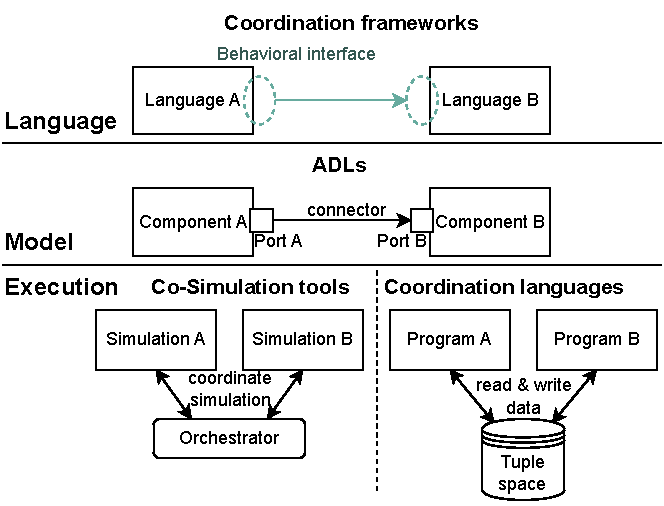
\includegraphics[width=1\textwidth]{images/overview}
	\caption{Overview of coordination approaches}
	\label{fig: overview}
\end{figure}

% Execution level
\textbf{Execution level:} Approaches on the \textit{execution level} aim to deal with coordination by interfacing directly with executable binaries or source code.
We identified two distinct categories on this level: co-simulation approaches and coordination languages.

% Short definition co-simulation and pointer
\textit{A co-simulation approach} composes the simulation of multiple components into a global simulation using an \textit{orchestrator}~\cite{gomesCoSimulationSurvey2019}.
A component simulation is typically given by an executable binary conforming to a predefined interface.
Co-simulation approaches are described in detail in \autoref{subsec: cosim}.

% Short definition coordination languages and pointer
\textit{A coordination language} provides a language and infrastructure, usually a communication \textit{medium}, to communicate and synchronize between components potentially executing on different machines.
Usually, coordination languages are integrated with programming languages, effectively adding coordination operations to the languages.
Coordination languages are described in detail in \autoref{subsec: coordlang}.

% Model level
\textbf{Model level:}
An \textit{Architecture Description Language (ADL)} operates on the \textit{model} level, i.e., each \textit{component} is given by a behavioral model, for example, a process algebra.
Components are then coordinated by linking them with \textit{connectors}, resulting in a \textit{configuration}.
ADLs are described in detail in \autoref{subsec: adl}.

% Language level
\textbf{Language level:}
\textit{Coordination frameworks} operate on the language level since they allow coordination of models conforming to \textit{different} behavioral languages using the concept of \textit{behavioral interfaces}.
They allow modelers to utilize different languages for varying aspects of the system.
Coordination frameworks are described in detail in \autoref{subsec: frameworks}.

\subsection{Co-simulation approaches} \label{subsec: cosim}

Julien will make a proposition.

\subsection{Coordination languages} \label{subsec: coordlang}
% Define Coordination language and give examples
Many different styles of coordination languages exist, which achieve coordination between components differently.

% Operation-based coordination languages
Coordination languages such as Linda~\cite{carrieroLindaContext1989} provide a \textit{set of operations} to enrich a host programming language with coordination capabilities.
The operations in Linda are used to read from and write to a virtual shared memory, which serves as a \textit{global} communication medium.
Such coordination languages are often called \textit{tuple-based} because the shared memory contains sequences of elements, i.e., tuples.
Ttuple-based coordination languages such as Linda are surveyed in \cite{rossiTuplebasedTechnologiesCoordination2001,nixonTuplespacebasedComputingSemantic2008,omiciniCoordinationModelsLanguages2011}.

% Channel-based coordination languages: REO, Manifold?
Other coordination languages such as Manifold~\cite{arbabOverviewManifoldIts1993,papadopoulosModellingActivitiesInformation1998} and REO~\cite{arbabReoChannelbasedCoordination2004} do not rely on a global communication medium but rather use \textit{channels} to connect components locally.
Each component then uses I/O operations to interact with connected channels without knowing who has sent or will receive data through the channel.
These coordination languages share many ideas with Architecture Description Languages (ADLs) discussed in the next section.

% Reactor-based coordination in Lingua Franca.
Finally, coordination languages might also use communication models such as the actor or reactor~\cite{lohstrohReactorsDeterministicModel2020} model.
For example, the Lingua Franca~\cite{lohstrohReactorsDeterministicModel2020,lohstrohLinguaFrancaDeterministic2021} coordination language is described using the reactor model, meaning one defines coordination by describing how each component reacts to incoming events.
A reaction to an event in one component might trigger reactions in connected components.
To encode reactions, the user can choose an existing programming language, such as C, C\texttt{++}, Python, TypeScript, and Rust.
Lingua Franca aims to simplify developing multi-threaded applications using the reactor model to guarantee \textit{determinism} and provide \textit{built-in timing semantics}.

\subsection{Architecture description languages} \label{subsec: adl}
% General idea
Architecture Description Languages (ADLs) aim to describe the structure of systems, allowing developers to focus on high-level components and their connections rather than lines of source code~\cite{clementsSurveyArchitectureDescription1996,medvidovicClassificationComparisonFramework2000,medvidovicFrameworkClassifyingComparing1997}.
% What is an ADL, and what is not?
Many different ADLs have been proposed in the academic literature and by the industry~\cite{medvidovicClassificationComparisonFramework2000,woodsArchitectureDescriptionLanguages2005}.
Nevertheless, clearly defining ADLs is challenging due to overlap with general-purpose modeling languages~\cite{clementsSurveyArchitectureDescription1996}.
For this paper, we consider only ADLs that incorporate formal semantics and thus do not consider other modeling languages such as UML~\cite{objectmanagementgroupUnifiedModelingLanguage2017} and ArchiMate~\cite{theopengroupArchiMateSpecification2023}.

% Describing ADLs generally.
The three buildings blocks of ADLs are defined as (1) \textit{components}, (2) \textit{connectors}, (3) \textit{architectural configuration}~\cite{medvidovicClassificationComparisonFramework2000,medvidovicFrameworkClassifyingComparing1997}.
% Component
A \textit{component} is a unit of computation or data repository~\cite{medvidovicClassificationComparisonFramework2000}.
Components vary in size, ranging from representing individual services to entire systems.

% Connector
\textit{Connectors} serve as architectural elements to model interactions between components and the regulations that oversee those interactions~\cite{medvidovicClassificationComparisonFramework2000}.
A difference to components is that connectors must not be implemented as distinct entities such as message brokers but can also represent shared variables or links between applications realized by client-server protocols~\cite{medvidovicClassificationComparisonFramework2000}.

% Architectural configuration
\textit{Architectural configuration}, also known as topology, represents the structural arrangement of components and connectors in a connected graph, defining the overall architecture~\cite{medvidovicClassificationComparisonFramework2000}.
This structure determines if the combined semantics results in the desired behavior.
For example, one can check for properties such as deadlocks and starvation.

% ADLS are formal and usually incorporate one formal language. Usually, a process algebra. They do not support multiple formal specification languages cite medvidovicClassificationComparisonFramework2000.
In addition, ADLs incorporate a formal language to enable formal analysis of specific properties.
The first ADLs were developed in the 90s and use process algebras such as Communicating Sequential Processes (CSP), Calculus of Communicating Systems (CCS), and $\pi$-calculus~\cite{ozkayaAreWeThere2013}.
For example, Wright uses CSP~\cite{allenFormalBasisArchitectural1997} while Darwin uses $\pi$-calculus~\cite{mageeSpecifyingDistributedSoftware1995}.
More recent ADLs, such as MontiArc~\cite{haberMontiArcArchitecturalModeling2014}, use automata to define the behavior of components.

However, no ADL supports heterogeneous components such as the coordination frameworks discussed in the next section~\cite{medvidovicClassificationComparisonFramework2000}.
Furthermore, despite the creation of numerous ADLs in the literature, they are not mainstream, i.e., not often used by practitioners in the industry~\cite{clementsSurveyArchitectureDescription1996,woodsArchitectureDescriptionLanguages2005,pandeyArchitecturalDescriptionLanguages2010,ozkayaAreWeThere2013,medvidovicMovingArchitecturalDescription2006}.

\subsection{Coordination frameworks} \label{subsec: frameworks}

Julien will make a proposition, which should include somewhere:

% Introduce the name of our approach
In this paper, we will refer to our methodology outlined in~\cite{krauterBehavioralConsistencyMultimodeling2023} as the \textit{Behavioral Coordination Language} (BCoorLang) to enhance clarity in communication.

\section{Methodology}
First, we conducted a \textit{meta-analysis} (tertiary study) on surveys (secondary studies) within each coordination category.
We found the following  secondary studies for coordination languages (\cite{papadopoulosCoordinationModelsLanguages1998,goosCoordinationModelsLanguages2001,rossiTuplebasedTechnologiesCoordination2001}), ADLs (\cite{clementsSurveyArchitectureDescription1996,medvidovicClassificationComparisonFramework2000,hussainInvestigatingArchitectureDescription2013,ozkayaAreWeThere2013,malavoltaWhatIndustryNeeds2013}), and co-simulation approaches (\cite{gomesCoSimulationSurvey2019,schweigerEmpiricalSurveyCosimulation2019,hafnerOverviewStateArt2021}).
We did not find surveys on coordination frameworks since the term is not yet commonly used.
We used Google Scholar to locate these papers, utilizing the keywords \quotes{survey}, \quotes{feature model}, \quotes{taxonomy}, and for each category, \quotes{coordination language}, \quotes{architecture description language}, or \quotes{co-simulation} accordingly.
We state our exact search queries in~\cite{timkrauterArtifactsCoordination2024}.
We then collected the first five pages of papers and filtered them by title, abstract, and content to arrive at the previously listed papers.

Second, we investigated individual approaches in each category to construct our taxonomy.
Due to the immense number of approaches and limited time, we focus on the 16 approaches listed in \autoref{sec: application}.
Our selection of these approaches is based on a mix of different criteria: distribution across categories, expert knowledge of the authors regarding relevance, and heterogeneity inside categories.
For example, we chose heterogeneous coordination languages, namely Linda, Reo, and Lingua Franca, which employ different coordination models, namely tuple spaces, channels, and reactors.

Finally, we refined our taxonomy by examining the secondary studies and individual coordination approaches until it reached a stable state described in the next section.

\section{Taxonomy} \label{sec: taxonomy}
We represent our taxonomy as a \textit{feature model}~\cite{kangFeatureOrientedDomainAnalysis1990}.
% TODO: Motivation is here again. It should be changed and more fitting
The aim is to compare coordination approaches from different categories.
It cannot contain all the details from each approach since it must operate on a higher abstraction level to allow comparison across categories.
Thus, it can be too coarse-grained to compare approaches inside the same category.
For example, if one only wants to compare co-simulation approaches, the feature model might not distinguish them enough.
Consequently, one should use a taxonomy created only for co-simulation, such as~\cite{gomesCoSimulationSurvey2019} instead.
However, our feature model still answers important questions.
For example, how can coordination be specified, and what is its semantics?
What are the goals of a coordination approach, how is the coordination implemented, and for which system domains is it suitable?

The top level of the feature model is shown in \autoref{fig: featureModelOverview}.
A coordination approach has three main features: \textit{Foundation}, \textit{Goal}, and \textit{Properties}.

\begin{figure}[ht]
	\centering
	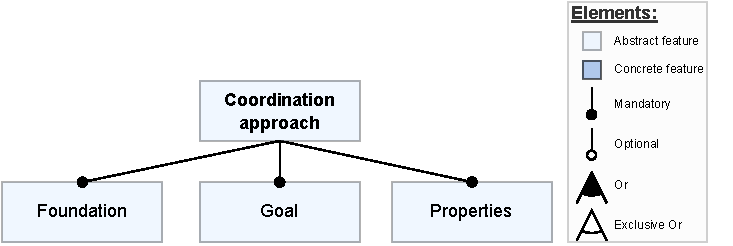
\includegraphics[width=0.85\textwidth]{images/root}
	\caption{Feature model overview}
	\label{fig: featureModelOverview}
\end{figure}

In the following sections, we will describe each abstract feature in detail.
% TODO: Update the full feature model when it is stable.
A complete diagram of the feature model is contained in~\cite{timkrauterArtifactsCoordination2024}.

\subsection{Foundation}

\autoref{fig: foundationFeature} shows the \textbf {Foundation} feature, which consists of \textbf{Definition}, \textbf{Mechanism}, and \textbf{Semantics}.

% Maybe cut into two pieces. So, Definition and Semantics are not part of the same.
\begin{figure}[ht]
	\centering
	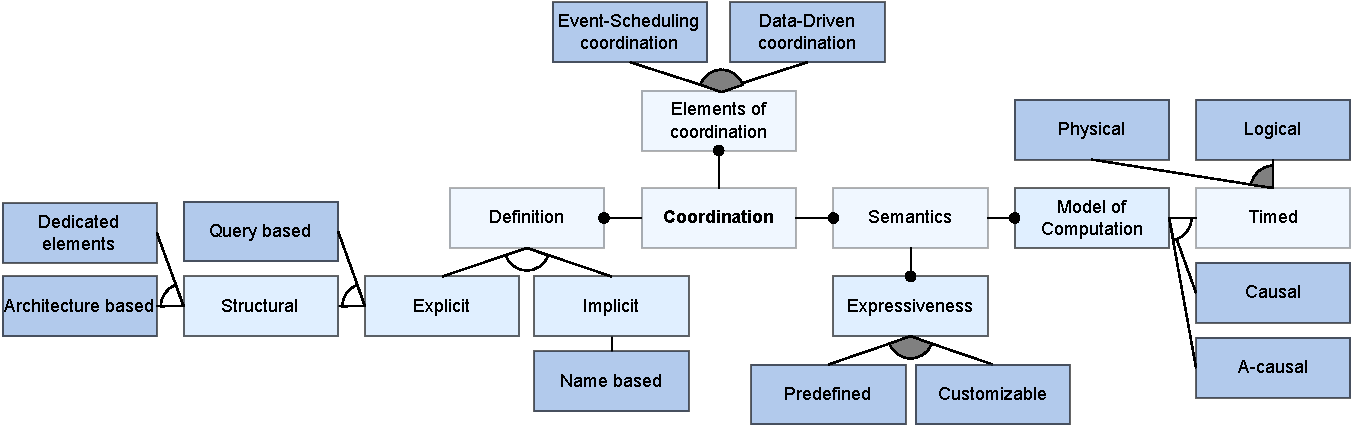
\includegraphics[width=1\textwidth]{images/coordination_feature}
	\caption{Foundation feature}
	\label{fig: foundationFeature}
\end{figure}

\subsubsection{Definition} The definition of coordination can either be \textit{explicit} or \textit{implicit}.
An implicit definition is usually based on the names of model elements.
For example, one could synchronize transitions of multiple state machines if they have identical names.

Explicit definition is either \textit{query based} or \textit{structural}.
% Query-based example
For example, in BCOoL~\cite{varalarsenBCOolBehavioralCoordination2016,varalarsenBehavioralCoordinationOperator2015}, one can write queries to define which elements should coordinate.

A structural definition of coordination uses \textit{dedicated elements} or is \textit{architecture based}.
For example, interactions in BCoorLang are specified by picking dedicated elements that should be coordinated, while coordination in ADLs depends on the architectural configuration~\cite{medvidovicClassificationComparisonFramework2000}, i.e., how ports of components are connected.

\subsubsection{Mechanism} The main mechanism driving coordination can be \textit{event scheduling}, \textit{data exchange}, or a mix of both.
In the literature, these mechanisms are sometimes also called control-driven or data-driven, respectively~\cite{papadopoulosCoordinationModelsLanguages1998,varalarsenBCOolBehavioralCoordination2016}.

First, \textit{event scheduling} synchronizes events or mandates a specific event order, i.e., order of state changes in different components.
Usually, event scheduling is used when components are given by behavioral models since there might not be a clear concept of an event in a programming language.
For example, in BCOoL~\cite{varalarsenBehavioralCoordinationOperator2015}, one can define relationships between events, such as \textit{happens before} or \textit{synchronize}.

\textit{Data-exchange} means components communicate by exchanging data.
For example, in the ADL MontiArc~\cite{haberMontiArcArchitecturalModeling2014}, components send data from the output to the input port.
Data can also be exposed as variables, which are then coupled with variables in other components, for example, to be the same. % Causal vs. A-causal MoC
However, data exchange might also happen between components during the synchronization of events, which is why both coordination mechanisms can be supported simultaneously.

\subsubsection{Semantics} The semantics feature consists of \textit{expressiveness} and \textit{model of computation}.
The expressiveness of coordination can be \textit{predefined}, i.e., a user has a fixed set of coordination mechanisms.
Expressiveness is \textit{customizable} if one can define the semantics of coordination.
For example, in BCOoL, one can employ the Clock Constraints Specification Language (CCSL)~\cite{andreSyntaxSemanticsClock2009} to define new coordination operators besides the predefined ones~\cite{varalarsenBCOolBehavioralCoordination2016,varalarsenBehavioralCoordinationOperator2015}.

Coordination approaches utilize different \textit{models of computation} (MoC).
A MoC is a set of rules that governs the concurrent execution and coordination of components~\cite{ptolemaeusSystemDesignModeling2014}.
We define three MoCs: \textit{timed}, \textit{causal}, \textit{a-causal}, where \textit{timed} is either \textit{physical} or \textit{logical}.
% Causal (data)
The \textit{causal} and \textit{a-causal} MoCs come from the co-simulation field~\cite{gomesCoSimulationSurvey2019}.
The causal MoC means that the coordination approach facilitates event and data exchange between different components such that one component can cause reactions, i.e., state changes in other components.
For example, a component based on a state machine raises an event, including data, which causes a state change and possible other reactions in a different component.

% A-causal
An a-causal MoC is necessary if one must deal with related differential equations.
For example, a variable in one equation should equal a variable in a different equation.
In this case, there is no cause and effect, such as in the causal MoC, but rather, the variables have an a-causal relationship since they should be equal at any time.

% Timed::Logical
\textit{Logical} time means that coordination approaches define when events/state changes happen.
Typically, one defines that events take place simultaneously or that one event causes another event immediately or with a fixed delay.
For example, a delay could be 50 milliseconds of logical time, corresponding to time in a simulation that can run arbitrarily fast.

% Timed::Physical
In contrast, \textit{physical} time describes time passing in the physical world.
It is also referred to as \textit{wall-clock} time~\cite{gomesCoSimulationSurvey2019}.
For example, one can define that an event should happen 50 milliseconds after another.
In Lingua Franca~\cite{lohstrohReactorsDeterministicModel2020}, logical time \quotes{chases} physical time, i.e., logical time tries to match the physical time provided by the execution platform.
% Logical time, however, always lags behind physical time.


\subsection{Goal} % Or even call it motivation
We identified three different \textit{goals} of coordination approaches: \textbf{simulation}, \textbf{execution}, and \textbf{formal validation}, see \autoref{fig: goalFeature}.
A coordination approach can have one or multiple goals, which we will now describe in detail.

\begin{figure}[ht]
	\centering
	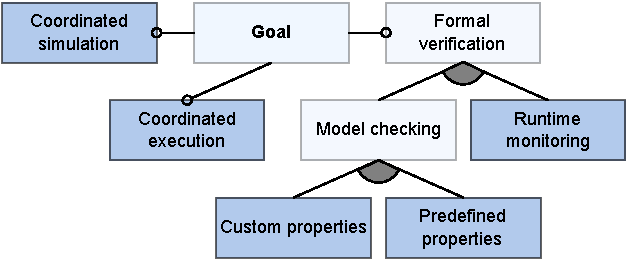
\includegraphics[width=0.7\textwidth]{images/goal_feature}
	\caption{Goal feature}
	\label{fig: goalFeature}
\end{figure}

\subsubsection{Simulation} The most common goal of coordination approaches is a coordinated simulation of multiple components or behavioral models representing an entire system.
A coordinated simulation is useful because the composition of multiple components can lead to unexpected behavior, often called \textit{emergent behavior}~\cite{ekerTamingHeterogeneityPtolemy2003}.
Emergent behavior can be dealt with early in development before implementing each component and its interactions.
Co-simulation approaches such as DACCOSIM~\cite{galtierFMIBasedDistributedMultisimulation2015,dadSynthesisFeedbackDistribution2021} or MECSYCO (Multi-agent Environment for ComplexSYstem CO-simulation)~\cite{camusHybridCosimulationFMUs2016,camusCosimulationCyberphysicalSystems2018} are examples of approaches that have coordinated simulation as their goal.
Simulation is also a goal of coordination frameworks such as BCoorLang~\cite{krauterBehavioralConsistencyMultimodeling2023} and BCOol~\cite{varalarsenBehavioralCoordinationOperator2015}.
Even recent ADLs such as MontiArc~\cite{haberMontiArcArchitecturalModeling2014} provide simulation capabilities.

\subsubsection{Execution} In contrast to coordinated simulation, which often only aims to find errors during development, some coordination approaches aim to provide a coordination infrastructure for system execution upon deployment.
For example, Linda provides a virtual shared memory with read and write operations to coordinate components.

Furthermore, the recently developed polyglot coordination language \textit{Lingua Franca} provides determinism guarantees during distributed execution~\cite{lohstrohLinguaFrancaDeterministic2021}.
Thus, it aims to provide a better coordination framework for concurrent \textit{execution}.


\subsubsection{Formal validation} Another goal of coordination approaches, especially for safety-critical systems, is formal validation of the coordinated system.

We encountered coordination approaches that validate \textit{predefined properties}, while others support \textit{custom properties}.
% (Definition 5)
For example, the ADL Wright~\cite{allenFormalBasisArchitectural1997} can check \textit{deadlock freedom} of component interactions.
% Darwin and we are checking custom properties: mageeBehaviourAnalysisSoftware1999 krauterBehavioralConsistencyMultimodeling2023
The coordination framework for behavioral consistency~\cite{krauterBehavioralConsistencyMultimodeling2023} supports custom properties written in temporal logic such as Linear Temporal Logic (LTL) and Computational Tree Logic (CTL).

\subsection{Properties}
We identified several reoccurring properties when analyzing coordination approaches.
\autoref{fig: propertiesFeature} depicts the resulting \textit{properties} feature, which we will now explain in detail.

\begin{figure}[ht]
	\centering
	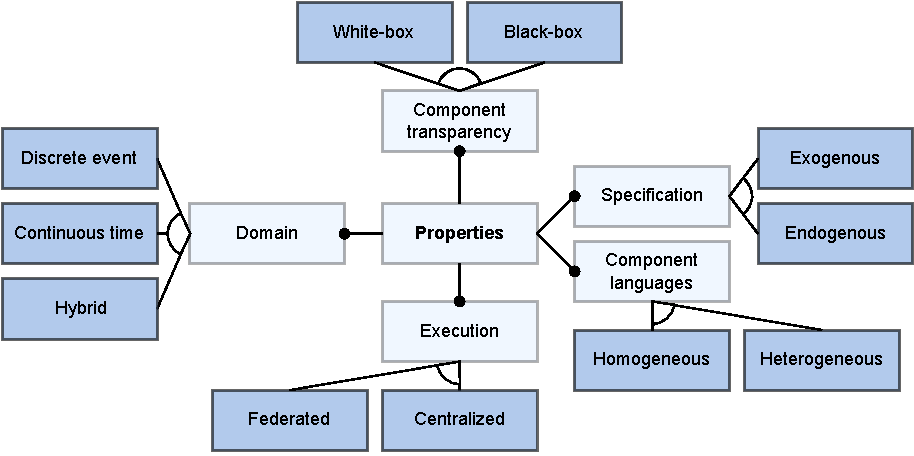
\includegraphics[width=1\textwidth]{images/properties_feature}
	\caption{Properties feature}
	\label{fig: propertiesFeature}
\end{figure}

% Maybe add some examples and descriptions here.
\subsubsection{Domain} Coordination approaches operate in different domains like the domains of co-simulation approaches described in~\cite{gomesCoSimulationSurvey2019}.
First, if a coordination approach is part of the \textit{Discrete event} (DE) domain, it allows discrete but not continuous state changes~\cite{gomesCoSimulationSurvey2019}.
Typically, coordination frameworks and ADLs operate in the DE domain since variables change their values discontinuously during execution, i.e., immediately change between states.
% discrete = discontinuous

Second, coordination approaches in the \textit{continuous time} (CT) domain support components to have a state that evolves continuously over time.
Often, components are given by differential equations, which induce continuous variable changes, such as physical systems involving springs and dampeners, see~\cite{gomesCoSimulationSurvey2019}.

Third, the \textit{hybrid} domain is a mix of the DE and CT domains that occur, for example, when simulating cyber-physical systems.
In a hybrid domain, components should coordinate where some change their state discretely (DE domain) while others evolve continuously over time (CT domain).
% MECSYCO is doing the first, while DACCOSIM is doing the second
Two strategies deal with hybrid systems: either adapt the components from the CT to the DE domain or vice versa~\cite{gomesCoSimulationSurvey2019}.

% TODO: Move somewhere appropriate.
% The choice of a coordination approach depends on the nature of the system at hand.
% For instance, software systems can usually be modeled in the discrete event domain, while physical or cyber-physical systems operate in the continuous time or even hybrid domain.

\subsubsection{Implementation} Coordination approaches are implemented differently.
Most approaches are implemented using \textit{general-purpose languages}.
For example, Linda is implemented in multiple languages such as C, C\texttt{++}, Java, and more, while Ptolemy is implemented in Java~\cite{ptolemaeusSystemDesignModeling2014}. 

Alternatively, a coordination approach can be implemented in a \textit{formal language}, which can then be run on an execution engine implemented for that formalism.
For example, the coordination framework BCoorLang~\cite{krauterBehavioralConsistencyMultimodeling2023} uses graph or term-rewriting as formal languages to coordinate heterogeneous components in a centralized manner.
It relies on the graph-transformation tool Groove~\cite{rensinkGROOVESimulatorTool2004} or the term-rewriting tool Maude for execution.

\subsubsection{Component transparency} Some coordination approaches require components to be entirely transparent (\textit{white-box}), while others only require a fixed interface (\textit{black-box}).
Usually, black-box approaches are needed to protect \textit{intellectual property} (IP) when different companies want to work together without sharing all the details concerning their components.
% TODO: Add a white-box a-causal example. Julien link or co-sim survey? 

For example, DACCOSIM only requires each component to conform to the FMI specification for Co-Simulation.

\subsubsection{Specification} We distinguish between \textit{endogenous} and \textit{exogenous} specification of coordination, as described for coordination languages in~\cite{arbabWhatYouMean1998}.
For example, when using the coordination language Linda~\cite{carrieroLindaContext1989}, one uses basic operations such as \textsf{out} and \textsf{in} inside components to write to and read from shared tuple space, i.e., shared memory.
Thus, Linda is \textit{endogenous} since one has to add coordination operations inside the components.

On the other hand, \textit{exogenous} coordination approaches keep coordination aspects outside of components.
However, components must still be created with coordination in mind to expose possible coordination points.
For example, BCOol~\cite{varalarsenBehavioralCoordinationOperator2015} uses behavioral interfaces to define events, which can then be used to specify \textit{exogenous} coordination rules outside the components.
Endogenous coordination approaches tend to mix computation and coordination~\cite{arbabWhatYouMean1998}.

\subsubsection{Component languages} Coordination approaches typically only support \textit{homogeneous} components.
For example, coordination languages, such as Lingua Franca~\cite{lohstrohReactorsDeterministicModel2020}, only support coordination if each component is given in the same programming language.

Similarly, most ADLs only coordinate components defined using the same modeling language.
As stated earlier, ADLs often use a specific process algebra to define the behavior of its components.
However, coordination frameworks allow \textit{heterogeneous} components, i.e., components specified in different behavioral modeling languages.
For example, BCoorLang~\cite{krauterBehavioralConsistencyMultimodeling2023} supports all modeling languages where one can clearly define \textit{state structure} and which \textit{elements can change state} during execution.

\subsubsection{Execution} A coordination approach is realized using either a \textit{centralized} or \textit{federated} execution.
In a \textit{centralized} execution, all components are executed by one engine, which enforces coordination.
For example, BCorrLang composes the behavior of all component specifications into a global behavior specification, which is then executed by a graph transformation or term-rewriting tool.

On the other hand, in a \textit{federated execution}, components run independently and only coordinate using a shared infrastructure through predefined connections.
Federated execution can still happen on the same physical machine, i.e., it does not mean that components must be \textit{distributed} across different physical machines. 

For example, the coordination language Lingua Franca~\cite{lohstrohReactorsDeterministicModel2020} supports federated execution on one machine by providing a runtime infrastructure.
DACCOSIM~\cite{galtierFMIBasedDistributedMultisimulation2015} goes one step further and allows a \textit{distributed} federated execution.


\section{Application of the feature model} \label{sec: application}
\autoref{tab:classification} shows the application of our feature model to four different coordination approaches.
Each approach comes from a different category: co-simulation (\textit{DACCOSIM}~\cite{galtierFMIBasedDistributedMultisimulation2015,dadSynthesisFeedbackDistribution2021}), coordination language (\textit{Linda}~\cite{carrieroLindaContext1989,carrieroLindaAlternativeMessagepassing1994}), ADL (\textit{MontiArc}~\cite{haberMontiArcArchitecturalModeling2014}), and coordination framework (\textit{BCoorLang}~\cite{krauterBehavioralConsistencyHeterogeneous2021,krauterBehavioralConsistencyMultimodeling2023}).
% TODO: Why did we choose these? Representative feature sets?

In addition, we classified the 12 following approaches: Ptolemy~\cite{ekerTamingHeterogeneityPtolemy2003,ptolemaeusSystemDesignModeling2014}, Wright~\cite{allenFormalBasisArchitectural1997,allenFormalApproachSoftware1997}, CommUnity~\cite{fiadeiroSemanticsArchitecturalConnectors1997,oliveiraCommUnityWorkbench2007}, Metropolis~\cite{balarinMetropolisIntegratedElectronic2003}, UMoC\texttt{++}~\cite{mathaikuttyUMoCBasedMultiMoC2006}, Lingua Franca~\cite{lohstrohReactorsDeterministicModel2020,lohstrohLinguaFrancaDeterministic2021}, Reo~\cite{arbabReoChannelbasedCoordination2004}, BIP~\cite{bliudzeAlgebraConnectorsStructuring2008,basuRigorousComponentBasedSystem2011}, Manifold~\cite{arbabOverviewManifoldIts1993,papadopoulosModellingActivitiesInformation1998}, and ForSyDe~\cite{sanderSystemModelingTransformational2004,sanderForSyDeSystemDesign2016}.
Due to space constraints, we cannot show all classifications but the full data set is available in the artifacts of this paper~\cite{timkrauterArtifactsCoordination2024}.

\begin{table}
	\centering
	\caption{Approach classification}
	\label{tab:classification}
	\resizebox{\textwidth}{!}{
	\SetTblrInner{colsep=2pt}
	\begin{tblr}{
			column{2-Z} = {c},
			hline{1, 2, Z} = {-}{1.2pt, solid}, % Z is the last row/column
			hline{7, 11} = {-}{dashed},
			vline{2-Y} = {2-Z}{solid},
		}
		\diagbox[linewidth=1.1pt,font=\bfseries]{Feature}{Approach} & \textbf{DACCOSIM} & \textbf{Linda} & \textbf{MontiArc} & \textbf{BCoorLang} \\
		
		\textbf{Foundation} \\
		\hspace{2mm} Definition & Architecture based & Name based & Architecture based & Dedicated elements \\
		\hspace{2mm} Mechanism & Data-Exchange & Data-Exchange & Data-Exchange & Event-Scheduling \\
		\hspace{2mm} Expressiveness & Predefined & Predefined & Predefined & Predefined \\
		\hspace{2mm} MoC & Causal & Causal & Logical, Causal & Logical \\
		
		\textbf{Goal} \\
		\hspace{2mm} Simulation & + & - & + & + \\
		\hspace{2mm} Execution & - & + & - & - \\
		\hspace{2mm} Formal verification & - & - & - & Custom properties \\
		
		\textbf{Properties} \\
		\hspace{2mm} Domain & Hybrid & Discrete event & Discrete event & Discrete event \\	
		\hspace{2mm} Implementation & GPL & GPL & GPL & Formal language \\
		\hspace{2mm} Comp. transparency & Black-box & White-box & White-box & White-box \\
		\hspace{2mm} Specification & Exogenous & Endogenous & Endogenous & Exogenous \\
		\hspace{2mm} Comp. languages & Homogeneous & Homogeneous & Homogeneous & Heterogeneous \\
		\hspace{2mm} Execution & Federated & Federated & Centralized & Centralized \\
	\end{tblr}
	}
\end{table}

We compare BCoorLang, MontiArc, and Linda in \autoref{fig: venn-bcoorlang-montiarc-linda}.
The figure shows a Venn diagram comparing the feature sets of each approach, where each colored part states which features are contained.
In addition, the number in the intersection states the amount of common features.

\begin{figure}[ht]
	\centering
	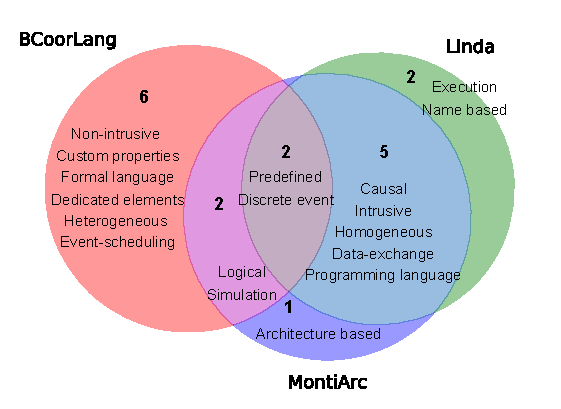
\includegraphics[width=0.6\textwidth]{images/venn_bcoorlang_montiarc_linda}
	\caption{Feature comparison: BCoorLang, MontiArc, and Linda}
	\label{fig: venn-bcoorlang-montiarc-linda}
\end{figure}

For example, the \textsf{1} at the bottom of \autoref{fig: venn-bcoorlang-montiarc-linda} describes that MontiArc has one \textit{original} feature (\textsf{Definition:Architecture based}), while the \textsf{3} in the intersection of all approaches in the middle declares that they all have three features in \textit{common} (\textsf{Expressiveness:Predefined, Domain:Discrete event, Component transparency:White-box}), see \autoref{tab:classification}.
All classification data and scripts to generate Venn diagrams such as \autoref{fig: venn-bcoorlang-montiarc-linda} are included in~\cite{timkrauterArtifactsCoordination2024}.

From \autoref{fig: venn-bcoorlang-montiarc-linda}, one can see that Linda has three original features compared to BCoorLang and MontiArc.
\textsf{Goal:Execution}, \textsf{Definition:Name based}, and \textsf{Execution:Federated} are not shared.
Furthermore, one can see that coordination frameworks, i.e., BCoorLang (the diagram is similar for BCOol~\cite{varalarsenBehavioralCoordinationOperator2015,varalarsenBCOolBehavioralCoordination2016}) greatly differ from ADLs and coordination languages.
Coordination frameworks have multiple unique features, such as \textsf{Component languages:Heterogeneous} and \textsf{Formal verification:Custom properties}.


Similarly, \autoref{fig: venn-bcoorlang-montiarc-daccosim} compares the features of BCoorLang and MontiArc with the co-simulation approach DACCOSIM.
One can see that BCoorLang and DACCOSIM do not have many features in common, probably due to their different goals as a coordination approach.
Co-simulation approaches like DACCOSIM have original features, such as \textit{Execution:Federated}, \textsf{Domain:Hybrid}, and \textsf{Component transparency:Black-box}.

\begin{figure}[ht]
	\centering
	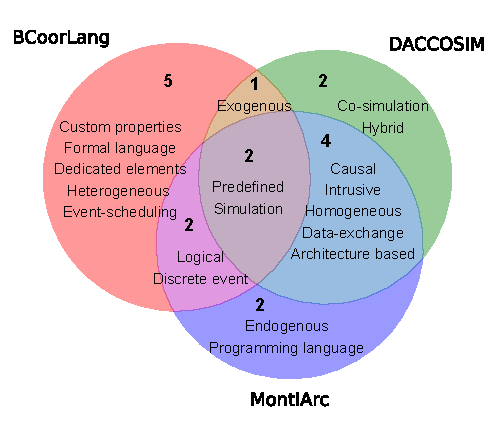
\includegraphics[width=0.6\textwidth]{images/venn_bcoorlang_montiarc_daccosim}
	\caption{Feature comparison: BCoorLang, MontiArc, and DACCOSIM}
	\label{fig: venn-bcoorlang-montiarc-daccosim}
\end{figure}

Venn diagrams such as \autoref{fig: venn-bcoorlang-montiarc-linda} and \autoref{fig: venn-bcoorlang-montiarc-daccosim} give a good approximation of the similarity between coordination approaches.
However, they do not tell the whole story since each feature is given the same importance, which is not entirely correct.
For example, a difference in the \textit{domain} feature might be more profound than another feature.

We stick to this simplification throughout this paper since the importance of features can be highly subjective.
In addition, we provide all data and scripts of our analysis as artifacts~\cite{timkrauterArtifactsCoordination2024}, which allows adapting the analysis to different needs in the future.

\section{Findings} \label{sec: findings}

We further analyze the classification of the 16 approaches, mentioned in \autoref{sec: application}, to find out how they compare across and inside the four categories.
We clustered the approaches to see similarities and differences by just looking at the feature data of each approach, not considering to which category they belong.
The data and scripts to reproduce our analysis are available in~\cite{timkrauterArtifactsCoordination2024}.
We apply a standard clustering algorithm using Jaccard distance to measure the similarity of the feature sets.
Jaccard distance is the one-complement of Jaccard similarity for two sets, defined as the ratio of their intersection to their union ~\cite{levandowskyDistanceSets1971}.
It is a widely used and reasonable dissimilarity measure for sets~\cite{levandowskyDistanceSets1971}.

\autoref{fig: clusters} shows a scatter plot with approximate positions of each approach derived solely from the distances between them.

\begin{figure}[ht]
	\centering
	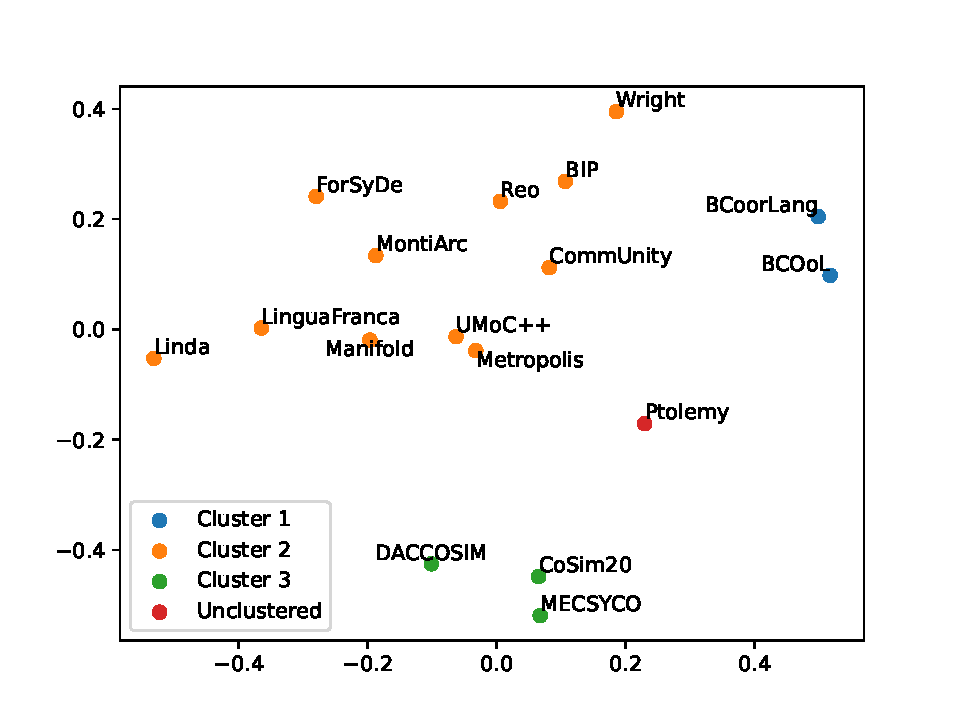
\includegraphics[width=1\textwidth]{images/approach_scatter}
	\caption{Feature distance and clustering of approaches}
	\label{fig: clusters}
\end{figure}

% TODO: Describe and interpret the scatter plot. Why is this interesting/new knowledge/insight? --> Blurs the lines between application and analysis. But I lean more towards analysis! --> Distances + clustering

% Add some low-level takeaways


% Interprete the previous classification
% Highlight typical features for ADLs, Coordination language, Co-simulation, and coordination frameworks.
% Are all ADLS similar? Any outliers?

% Commonalities between clusters

% Differences between clusters

% What are the unique features of each approach? Does this match their intended usage scenarios?

% ADLs, coordination languages, and coordination frameworks usually apply to software systems, while co-simulation applies to hybrid systems, i.e., cyber-physical systems. Thus, they support different MoCs and domains and have different goals.

% High-level takeaways
\textbf{Coordination frameworks do not support Data-Exchange:} All coordination frameworks we have encountered support \textsf{Event-Scheduling} but not \textsf{Data-Exchange} as a coordination mechanism.
This is likely because data exchange is difficult to achieve when heterogeneous components are allowed.
However, data exchange is omnipotent in real-world systems, so it is the main coordination mechanism used in co-simulation approaches and coordination languages.
Thus, for coordination frameworks to be employed in real-world scenarios, they must support data exchange.
Also, data exchange is identified as an important future work in works like ~\cite{krauterBehavioralConsistencyMultimodeling2023,varalarsenBCOolBehavioralCoordination2016}.

\section{Conclusion \& future work} \label{sec: conclusion}

\bibliographystyle{splncs04}
\bibliography{bib}

\end{document}
